\documentclass[hyperref,french,usenames,xcolor=dvipsnames]{beamer}
\mode<presentation>
{
\usepackage{beamerthemesplit}
\usetheme[compress,secheader]{Madrid}
%  \usecolortheme{orchid}
%       \setbeamercolor{alerted text}{fg=red!65!black}
  \setbeamercovered{transparent}
}
\usepackage{amsthm}
\usepackage{amsfonts}
\usepackage{amsmath}
\usepackage{graphicx}
%\usepackage{epsfig}
\usepackage{xspace}
\usepackage{stmaryrd}
%\usepackage{soul}
\usepackage[utf8]{inputenc}

\definecolor{newcolor}{rgb}{0, 0, .90}
\definecolor{impcolor}{rgb}{.90, 0, 0}
\definecolor{darkergreen}{rgb}{0,0.5,0}
\definecolor{myorange}{rgb}{0.8,0.7,0}
\definecolor{myviolet}{rgb}{0.7,0.0,0.7}

\definecolor{lightpurple}{rgb}{0.83,0.27,1}
\definecolor{lightblue}{rgb}{0.27,0.9,0.9}



%\newcommand{\texthl}[1]{{\color{blue}#1}}
%\newcommand{\jaune}[1]{{\color{blue}#1}}
%\newcommand{\texthlb}[1]{{\color{orange}#1}}
%\newcommand{\orange}[1]{{\color{orange}#1}}
%\newcommand{\verte}[1]{{\color{green}#1}}
%\newcommand{\trad}{{\color{orange}{\bf $\leadsto$}}}

%\newcommand{\textcite}[1]{{\color{lightpurple}[#1]}}
%\newcommand{\textciten}[1]{{\color{lightpurple}#1}}

\newcommand{\texthl}[1]{{\color{red}#1}}
\newcommand{\jaune}[1]{{\color{red}#1}}
\newcommand{\texthlb}[1]{{\color{orange}#1}}
\newcommand{\orange}[1]{{\color{orange}#1}}
\newcommand{\verte}[1]{{\color{green}#1}}
\newcommand{\trad}{{\color{orange}{\bf $\leadsto$}}}

\newcommand{\textcite}[1]{{\color{myviolet}[#1]}}
\newcommand{\textciten}[1]{{\color{myviolet}#1}}

\newcommand{\montilde}{$\sim$}


\title[SORBB]%
{Object Retrieval using a Bag of Boundaries}

\author{Vadim \textsc{Kantorov} \& \textsc{Nelle Varoquaux}}
\institute[ENS]{
\structure{
École Normale Supérieur de Cachan}
}

\date[09/12/11]{MVA - 09/12/11}

%\date[] % (optional)
%{}

\subject{Rencontres Mondiales du Logiciel Libre - 12/07/11}

\AtBeginSection[] % Do nothing for \section*
{
  \frame<beamer>
  {
    \frametitle{Sommaire}
    \tableofcontents[current]
  }
}

\begin{document}

\frame{\titlepage}

\section{Problematic}
\frame{
\frametitle{Problematic}

}
\section{The Segmentation}
\section{Smooth Objects Retrieval}
\frame{
\frametitle{Boundary Descriptors}
\begin{itemize}
  \item HOGs
  \item Occupancy grid
\end{itemize}

\begin{figure}[!t]
\centering
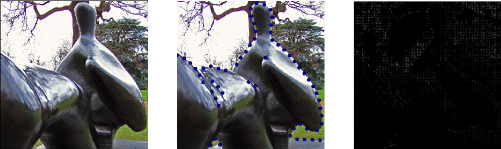
\includegraphics[height=80px]{./images/desc.png}
\end{figure}

}

\frame{
\frametitle{Bags of Boundaries and Vocabulary}
\begin{itemize}
  \item MiniBatchKMeans with $k=10000$

\end{itemize}
}

\frame{
\frametitle{Object retrieval and matching}
\begin{itemize}
  \item tf-idf score
\end{itemize}

\begin{figure}[!t]
\centering
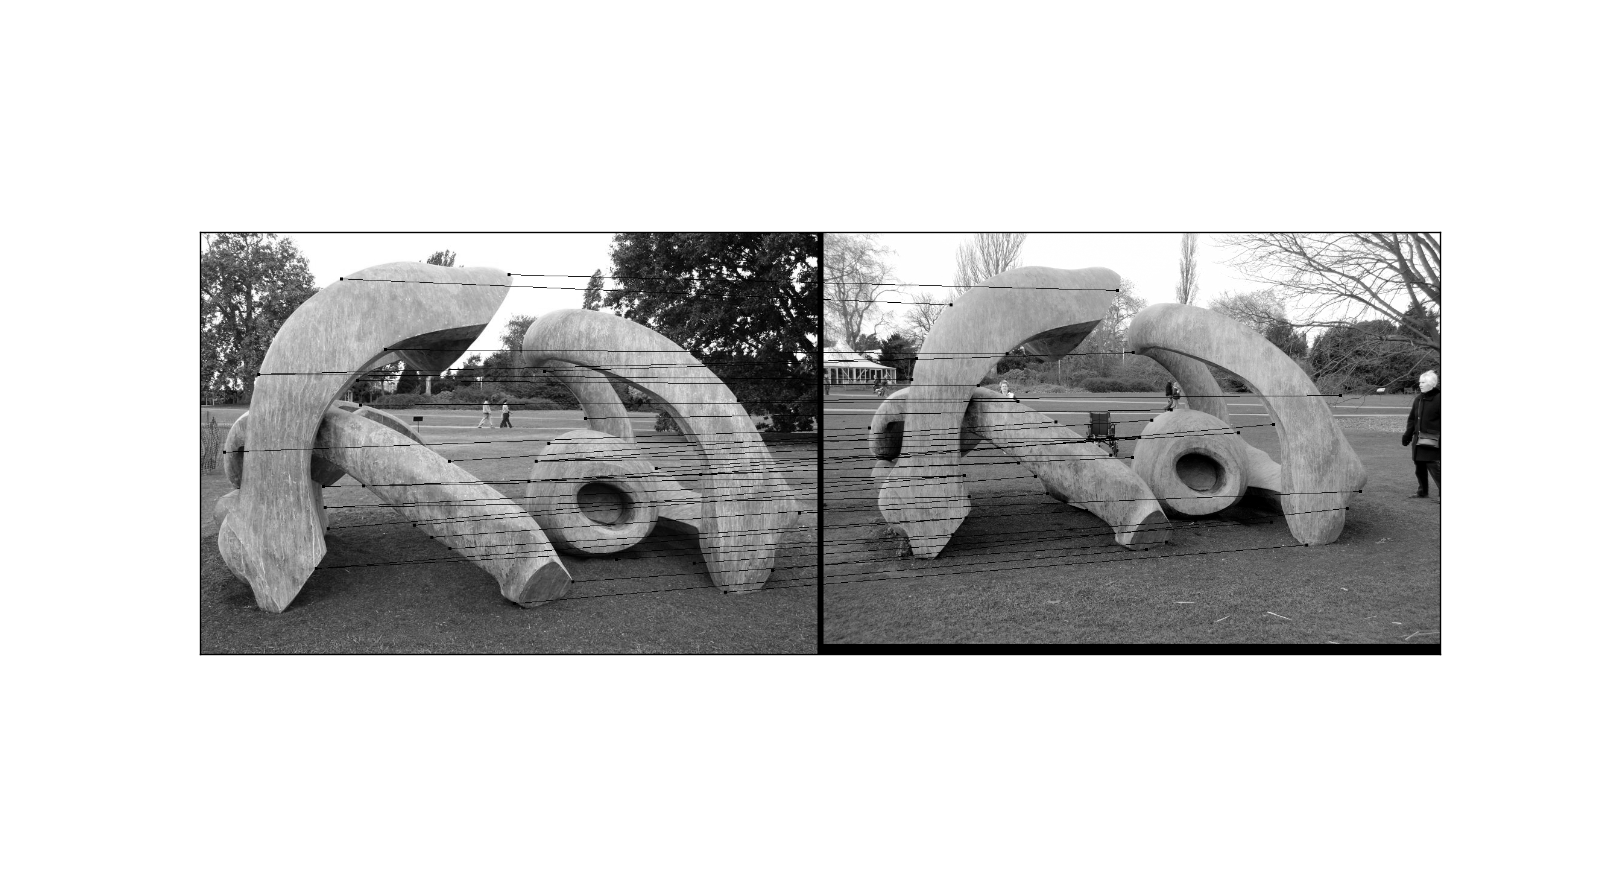
\includegraphics[height=150px]{./images/matching_01.png}
\end{figure}
}

\frame{
\frametitle{Results}
}
\section{Conclusion}

\end{document}
